\section{Method}\label{sec:method}

\subsection{Deterministic backbone (point reference)}
As a point-accuracy reference we train a deterministic regression backbone on the
rich feature vector with a mean-squared-error objective. The backbone is used
\emph{only} as the point-accuracy reference against which the CFM posterior's
point cost is measured; it produces no posterior and therefore cannot be
calibrated or ranked by confidence. Its accuracy is reported in
Section~\ref{sec:results}.

\subsection{Conditional flow-matching posterior}
The estimator of interest is a clean conditional flow-matching (CFM) model that
learns a velocity field transporting a \emph{cuboid-uniform bounded} base
distribution, $x_0\sim\mathrm{Unif}(\mathcal{C})$ over the phantom cuboid
$\mathcal{C}$, to the conditional distribution of capsule position given the
observed features; sampling starts from the same bounded base and integrates the
learned ODE with Euler updates, clamping every intermediate state to the cuboid
bounds. We use the ``clean'' configuration: independent-coupling CFM over a
shared vector-field backbone, exponential-moving-average weights with decay
$0.999$, and $200$ posterior samples per test point. Minibatch OT-CFM was
unstable on the small position-grouped batches, so it is not used for the
reported posterior. Figure~\ref{fig:method-cfm} summarizes the sampling pipeline.

\begin{figure*}[t]
\centering
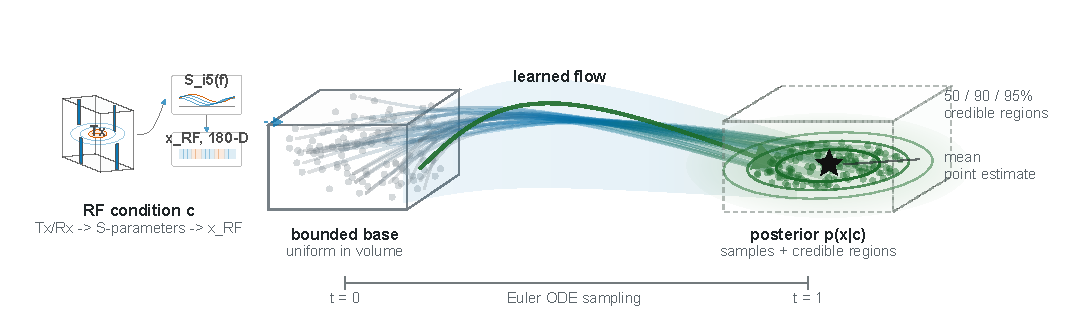
\includegraphics[width=0.96\linewidth]{figures/fig_method_cfm.pdf}
\caption{Conditional flow-matching posterior pipeline. The 180-D RF feature vector
conditions a velocity field $v_\theta(x,t\,|\,c)$ (FiLM blocks, EMA weights) that
transports cuboid-uniform bounded base samples to the conditional position
distribution; Euler ODE integration clamps each step to the cuboid bounds, and
200 draws form the empirical posterior, summarised by its mean (the point
estimate) and 50/90/95\% credible regions. \textbf{Simulation.}}
\label{fig:method-cfm}
\end{figure*}

\subsection{Formal CFM objective and training specification}
Let $c$ denote the normalized RF feature vector and $x_1\in\mathcal{C}\subset
\mathbb{R}^3$ the capsule position. Training draws a bounded base point
$x_0\sim\mathrm{Unif}(\mathcal{C})$ and $t\sim\mathrm{Unif}(0,1)$, then uses
the straight-line path
\begin{equation}
x_t=(1-t)x_0+t x_1,\qquad u_t=x_1-x_0,
\label{eq:cfm-path}
\end{equation}
% source: scripts/training/train_cfm_raw_rssi.py:552-568,570-584
with the conditional flow-matching loss
\begin{equation}
\mathcal{L}(\theta)=
\mathbb{E}_{(x_1,c),x_0,t}\left[
\left\|v_\theta(x_t,t\,|\,c)-u_t\right\|_2^2
\right].
\label{eq:cfm-loss}
\end{equation}
% source: scripts/training/train_cfm_raw_rssi.py:570-584
The implementation adds a small $\sigma_{\min}=0.001$\,m target jitter before
forming $x_1$ for training stability. At inference, each sample starts from the
same cuboid-uniform base and is advanced by clamped Euler integration,
\begin{equation}
\hat{x}_{k+1}=\Pi_{\mathcal{C}}\!\left[
\hat{x}_{k}+\Delta t\,v_\theta(\hat{x}_{k},k\Delta t\,|\,c)
\right],\qquad \Delta t=1/K ,
\label{eq:cfm-euler}
\end{equation}
% source: scripts/training/train_cfm_raw_rssi.py:608-638
where $\Pi_{\mathcal{C}}$ clips each coordinate to the cuboid bounds.

\begin{table}[t]
\centering
\caption{CFM architecture and training hyperparameters used for the reported posterior. \textbf{Simulation.}}
\label{tab:cfm-hparams}
\scriptsize
\setlength{\tabcolsep}{3pt}
\begin{tabular}{@{}p{0.38\linewidth}p{0.56\linewidth}@{}}
\toprule
Item & Value \\
\midrule
Dataset and folds & Combined rich dataset ($N=3935$); seeds $1,2,3$; $5$ position-grouped folds \\ % source: experiments/uq_bakeoff/cfm_uq_score_20260529_085917.json:410-416
Epoch schedule & $600$ epochs, patience $40$, validation every $5$ epochs \\ % source: experiments/uq_bakeoff/cfm_uq_score_20260529_085917.json:417-418; scripts/training/baselines/run_cfm_uq_score.py:274-303
Batch and optimizer & batch size $64$; AdamW, learning rate $2{\times}10^{-3}$, weight decay $10^{-4}$, betas $(0.9,0.95)$ \\ % source: scripts/training/baselines/run_cfm_uq_score.py:366-388; scripts/training/train_cfm_raw_rssi.py:526-549
Base and path & $x_0\sim\mathrm{Unif}(\mathcal{C})$; uniform $t$; linear path $x_t=(1-t)x_0+t x_1$; target $x_1-x_0$ \\ % source: scripts/training/train_cfm_raw_rssi.py:552-584
Stabilization & $\sigma_{\min}=0.001$\,m target jitter; gradient clipping at $1.0$ \\ % source: experiments/uq_bakeoff/cfm_uq_score_20260529_085917.json:425; scripts/training/train_cfm_raw_rssi.py:570-587
Coupling and weights & independent coupling (\texttt{use\_ot\_cfm=false}); EMA decay $0.999$ \\ % source: experiments/uq_bakeoff/cfm_uq_score_20260529_085917.json:426-428; scripts/training/train_cfm_raw_rssi.py:590-591
Sampling & Euler integrator, $K=50$ steps, $200$ posterior samples per test point \\ % source: scripts/training/baselines/run_cfm_uq_score.py:195-196,310-319; experiments/uq_bakeoff/cfm_uq_score_20260529_085917.json:429-430
Input split & leading $4$-D RSSI token stream plus $176$-D global rich-feature stream \\ % source: wce-cfm/Concepts/Rich feature set (180-D).html:35-38; scripts/training/baselines/run_cfm_uq_score.py:405-412
Vector-field width & hidden dimension $64$; $3$ FiLM residual blocks \\ % source: experiments/uq_bakeoff/cfm_uq_score_20260529_085917.json:419-420; scripts/training/train_cfm_raw_rssi.py:145-160,266-278
Attention and geometry & per-sensor geometry tokens with relative geometry; $4$-head self-attention; learned-query pooling; dropout $0.1$ \\ % source: scripts/training/train_cfm_raw_rssi.py:190-225,397-418
Feature/time embeddings & PLR feature embedding $K=24$, $\sigma=0.1$, $d=16$; Fourier time features $\sin/\cos(2\pi t,4\pi t,8\pi t,16\pi t)$ \\ % source: experiments/uq_bakeoff/cfm_uq_score_20260529_085917.json:421-424; scripts/training/train_cfm_raw_rssi.py:377-384
\bottomrule
\end{tabular}
\end{table}

\subsection{Posterior summaries and credible regions}
From the posterior sample cloud we form the empirical
posterior, report its mean as the point estimate, and construct credible regions
at nominal 50/90/95\% both as axis-aligned marginal boxes and as
Mahalanobis ellipsoids. \emph{Coverage} is the fraction of test points whose true
position lies inside the nominal region; \emph{discrimination} is the Spearman
correlation between posterior spread and realized error. A selective-prediction
(operating-point) view, in which the least-confident fraction of estimates is
deferred, follows directly from the spread ordering. Figure~\ref{fig:posterior-cloud}
shows the empirical sample representation used for these summaries.

\begin{figure}[t]
\centering
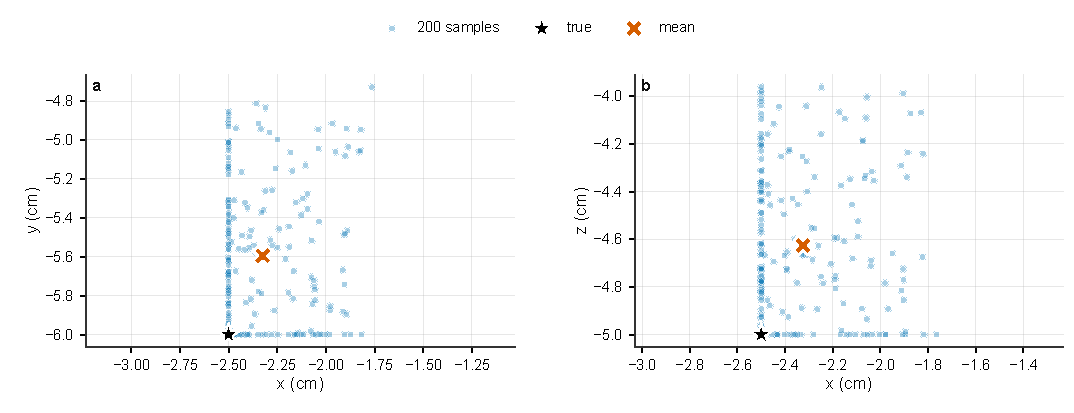
\includegraphics[width=0.9\linewidth]{figures/fig_posterior_cloud.pdf}
\caption{Example CFM posterior cloud for one test point, shown in the $x$--$y$
and $x$--$z$ projections. The 200 samples define the empirical posterior; the posterior mean is
the point estimate used for MAE, and the cloud spread defines the credible-region
and selective-prediction scores. \textbf{Simulation.}}
\label{fig:posterior-cloud}
\end{figure}

\subsection{Metrics}
For each held-out configuration $i=1,\ldots,N$, let $x_i$ be the true 3D
position, $\{s_i^{(m)}\}_{m=1}^{M}$ the posterior samples, and
$\bar{x}_i=M^{-1}\sum_m s_i^{(m)}$ the posterior mean. The 3D point metric is
\begin{equation}
\mathrm{MAE}_{3D}=\frac{1}{N}\sum_{i=1}^{N}\|\bar{x}_i-x_i\|_2 ,
\label{eq:mae3d}
\end{equation}
% source: scripts/training/baselines/run_cfm_uq_score.py:102-107; scripts/training/baselines/analyze_rich_benchmark.py:89-93
reported in centimetres. For nominal levels
$\alpha\in\{0.50,0.90,0.95\}$, let $q^{-}_{i,d}(\alpha)$ and
$q^{+}_{i,d}(\alpha)$ be the lower and upper sample quantiles on axis $d$.
Marginal and joint-box coverage are
\begin{align}
\mathrm{cov}_{\mathrm{marg}}(\alpha)
&=\frac{1}{3N}\sum_{i=1}^{N}\sum_{d=1}^{3}
\mathbf{1}\{q^{-}_{i,d}(\alpha)\le x_{i,d}\le q^{+}_{i,d}(\alpha)\},\\
\mathrm{cov}_{\mathrm{joint}}(\alpha)
&=\frac{1}{N}\sum_{i=1}^{N}
\mathbf{1}\{\forall d:\ q^{-}_{i,d}(\alpha)\le x_{i,d}\le q^{+}_{i,d}(\alpha)\}.
\label{eq:coverage}
\end{align}
% source: scripts/training/baselines/uq_metrics.py:155-202; scripts/training/baselines/run_cfm_uq_score.py:121-128
For a full-covariance Gaussian check, with local sample covariance $\Sigma_i$,
Mahalanobis-ellipsoid coverage is
\begin{equation}
\mathrm{cov}_{\mathrm{ell}}(\alpha)=\frac{1}{N}\sum_{i=1}^{N}
\mathbf{1}\{(x_i-\bar{x}_i)^\mathsf{T}\Sigma_i^{-1}(x_i-\bar{x}_i)
\le \chi^2_{3,\alpha}\}.
\label{eq:ellipsoid}
\end{equation}
% source: scripts/eval/cfm_v3_layer2_metrics.py:193-200,203-232
The sample CRPS is computed per axis and averaged,
\begin{align}
\mathrm{CRPS}
&=\frac{1}{3N}\sum_{i=1}^{N}\sum_{d=1}^{3}
\left[
\frac{1}{M}\sum_{m=1}^{M}|s_{i,d}^{(m)}-x_{i,d}|
\right. \notag\\
&\quad\left.
-\frac{1}{2M^2}\sum_{m,\ell=1}^{M}
|s_{i,d}^{(m)}-s_{i,d}^{(\ell)}|
\right],
\label{eq:crps}
\end{align}
% source: scripts/training/baselines/uq_metrics.py:33-77; scripts/training/baselines/run_cfm_uq_score.py:114-117
and the multivariate energy score is
\begin{align}
\mathrm{ES}
&=\frac{1}{N}\sum_{i=1}^{N}
\left[
\frac{1}{M}\sum_{m=1}^{M}\|s_i^{(m)}-x_i\|_2
\right. \notag\\
&\quad\left.
-\frac{1}{2M(M-1)}\sum_{m\ne \ell}\|s_i^{(m)}-s_i^{(\ell)}\|_2
\right].
\label{eq:energy}
\end{align}
% source: scripts/training/baselines/uq_metrics.py:105-148; scripts/training/baselines/run_cfm_uq_score.py:118-119
Sharpness is the mean posterior standard deviation over test points and axes,
\begin{equation}
\mathrm{sharpness}=\frac{1}{3N}\sum_{i=1}^{N}\sum_{d=1}^{3}
\mathrm{sd}_{m}\!\left(s_{i,d}^{(m)}\right).
\label{eq:sharpness}
\end{equation}
% source: scripts/training/baselines/uq_metrics.py:237-249; scripts/training/baselines/run_cfm_uq_score.py:134-139

\subsection{Orientation as a marginalized nuisance}
Capsule orientation in vivo is unknown and time-varying. We therefore treat
orientation as a nuisance variable to be \emph{integrated out}, not regressed.
Two mechanisms accomplish this: (i)~the backbone is approximately
orientation-invariant across the sampled poses, and (ii)~the CFM posterior's
\emph{width} absorbs the residual orientation-induced ambiguity.
Section~\ref{sec:results} quantifies the per-pose bias, the $180^\circ$
$y$-flip check, and how faithfully the posterior width tracks the
orientation-induced spread of the point estimate.

\subsection{Baselines}
Against the CFM posterior we evaluate: the deterministic backbone (point
reference); a 5-member deep ensemble; MC-dropout (50 samples); diagonal and
2-component mixture-density networks (MDN-diag, MDN-mix2; 200 samples); split
conformal applied to the deterministic backbone; and ten classical regressors
(HistGradientBoosting, ExtraTrees, RandomForest, SVR, NGBoost, $k$-NN, MLP,
AdaBoost, Ridge, and a fixed kernel Gaussian process). Every method is evaluated
on identical folds, seeds, and test indices.
